\documentclass [a4paper,12pt] {article}
\usepackage{fullpage}
\usepackage{graphicx}
\usepackage{hyperref}
\usepackage{color}
\usepackage{float}
\usepackage{caption}
\usepackage[font=small,skip=1pt]{caption}
\begin{document}
\begin{titlepage}
	\begin{center}
		\textsc{\huge\\[5cm] COS 301 - Mini Project}\\[1cm]
		\textsc{\huge Functional requirements and application design}\\[1cm]
		\textsc{\huge Group 1B}\\[1cm]
		\textsc{\large 2015}
	\end{center}
\end{titlepage}
\tableofcontents
\pagebreak
\section{Group Information}
	\subsection{General Information}
	We used Github as our version control service. The repository can be accessed at: \linebreak \url{https://github.com/thinusn/Mini-Project-Requirements-Group-1B}
	\subsection{Group members}
	\begin{itemize}
		\item 13033922 Elzahn Botha
		\item 12223426 Estian Rosslee
		\item 13025105 Jaco-Louis Kruger
		\item 13073878 Christopher Araüjo
		\item 13093500 Paul Engelke
		\item 13028741 Frikkie Snyman
		\item 13019602 Thinus Naude
	\end{itemize}
	\subsection{Contributions to project}
		\subsubsection{Participation}
		Estian Rosslee (12223426) only attended the two 1-hour meetings we had, \textbf{he did not do any of the work presented in this document.} All other members of the group participated fully towards completing the project.
		\subsubsection{Who did what}
			\begin{itemize}
				\item Planning: Everyone
				\item Use case prioritization: Everyone
				\item Services contracts: Jaco-Louis Kruger, Daniel Araüjo, Thinus Naude, Paul Engelke and Frikkie Snyman
				\item Required functionality: Jaco-Louis Kruger and Thinus Naude
				\item Process specifcations: Elzahn Botha, Daniel Araüjo, Paul Engelke
				\item Domain Model: Frikkie Snyman
				\item LaTex: Thinus Naude
			\end{itemize}
		\pagebreak
		\subsubsection{Github contribution}
		\begin{figure}[!htbp]
			\centering
			%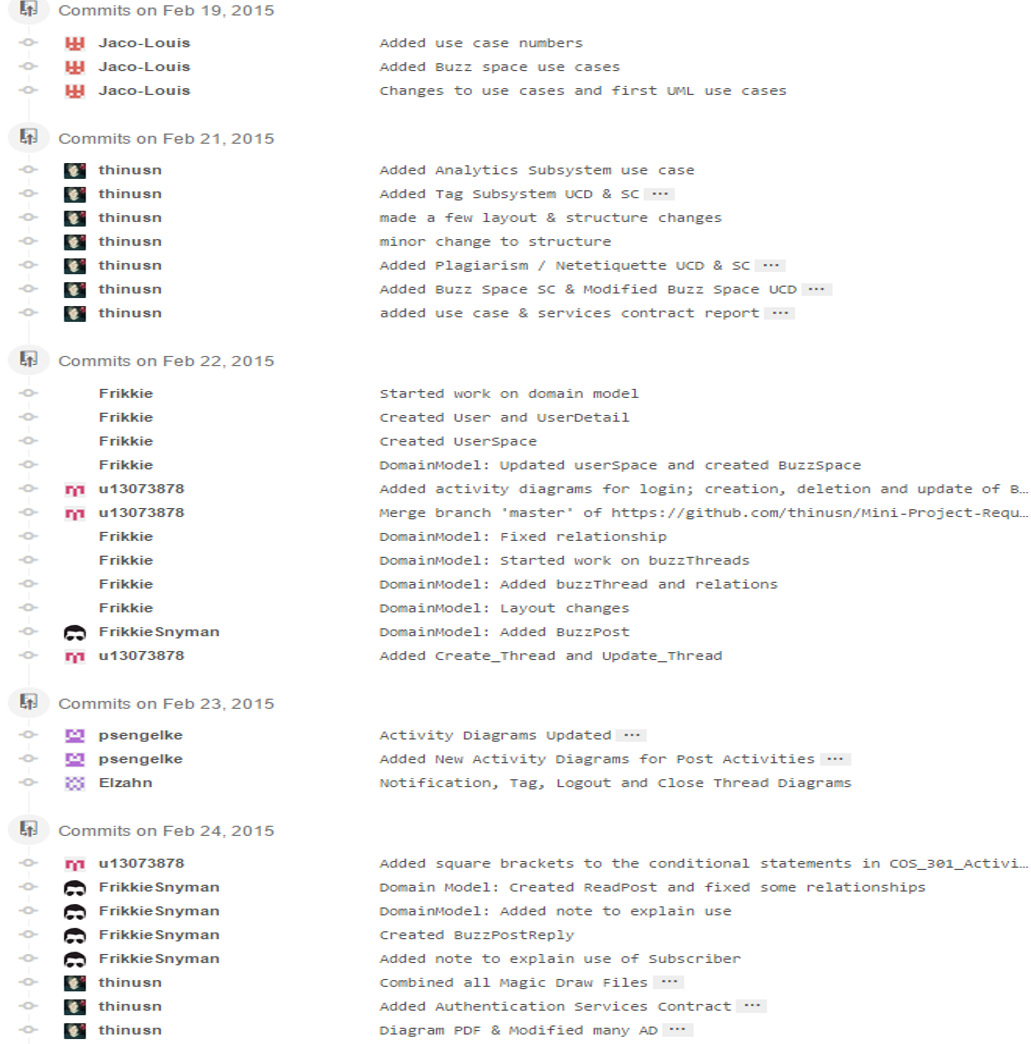
\includegraphics[width=1.0\textwidth]{githubCommits.png}
			\large\textbf{\colorbox{green}{IMAGE OF githubCommits}}
			\caption{Github pushes for project.}
		\end{figure}
\pagebreak
\section{Functional requirements and application design}
	\subsection{Use case prioritization}
	\subsubsection{Critical}A use case which is absolutely essential
	\begin{itemize}
		\item Create, Read/View/Get, Delete and Update of BuzzSpace
		\item Create, Read/View/Get, Delete and Update of Thread
		\item Create, Read/View/Get, Delete and Update of Thread Posts
		\item Authentication	
	\end{itemize}
	\subsubsection{Important}The system would still be useful without some of the important use cases, but the client would get quantifiably less value from the system.
		\begin{itemize}
			\item User (profiles and actions)
			\item User Communication (Email Templates)
			\item Tagging
		\end{itemize}
	\subsubsection{Nice-To-Have}Its a requirement but the value to the clientis insignificant.
		\begin{itemize}
			\item Plagiarism checker
			\item Netiquette checker
		\end{itemize}

\pagebreak
	\subsection{Services contracts}
		\subsubsection{Analytics}
			\begin{figure}[H]
				\centering
				%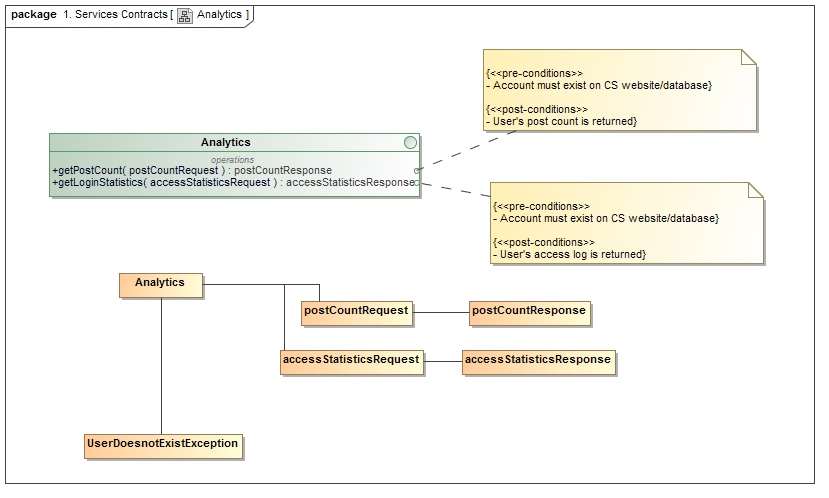
\includegraphics[width=1.0\textwidth]{AnalyticsSC.png}
				\large\textbf{\colorbox{green}{IMAGE OF AnalyticsSC}}
				\caption{Analytics services contracts.}
			\end{figure}
		\subsubsection{Authentication}
			\begin{figure}[H]
						\centering
						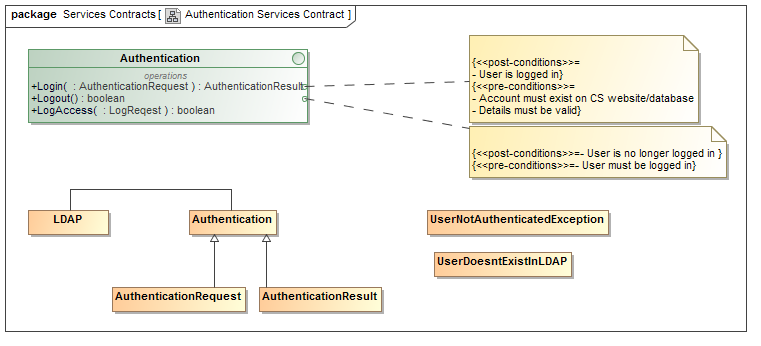
\includegraphics[width=1.0\textwidth]{AuthenticationSC.png}
						\caption{Authentication services contracts.}
			\end{figure}
		\subsubsection{BuzzSpace}
					\begin{figure}[H]
						\centering
						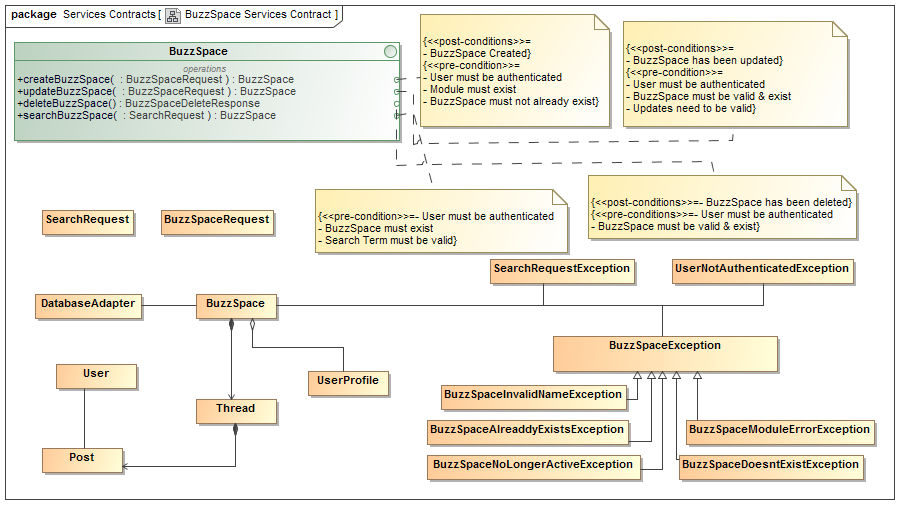
\includegraphics[width=1.0\textwidth]{BuzzSpaceSC.png}
						\caption{BuzzSpace services contracts.}
					\end{figure}
					
		\subsubsection{Communication}
			\begin{figure}[H]
				\centering
				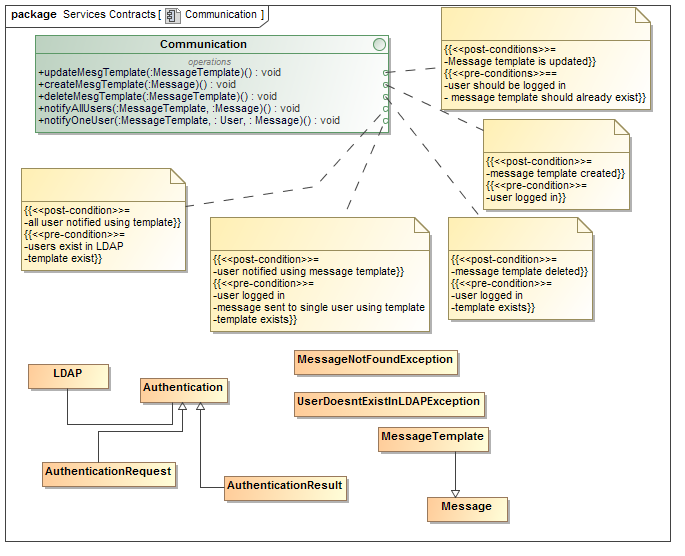
\includegraphics[width=1.0\textwidth]{CommunicationSC.png}
				\caption{Communication services contracts.}
			\end{figure}
		
		\subsubsection{Plagiarism / Netetiquette}
			\begin{figure}[H]
				\centering
				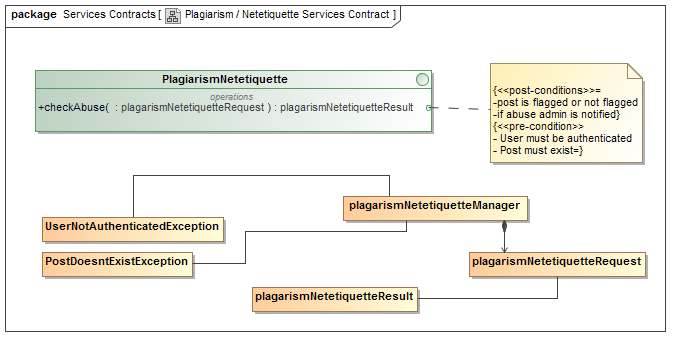
\includegraphics[width=1.0\textwidth]{PlagiarismNetetiquetteSC.png}
				\caption{Plagiarism and Netetiquette services contracts.}
			\end{figure}
		\subsubsection{Tagging}
			\begin{figure}[H]
				\centering
				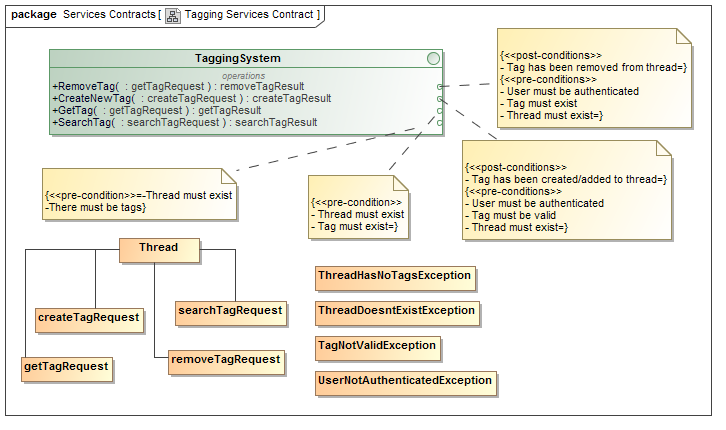
\includegraphics[width=1.0\textwidth]{TaggingSC.png}
				\caption{Tagging services contracts.}
			\end{figure}
		\subsubsection{Thread}
			\begin{figure}[H]
				\centering
				%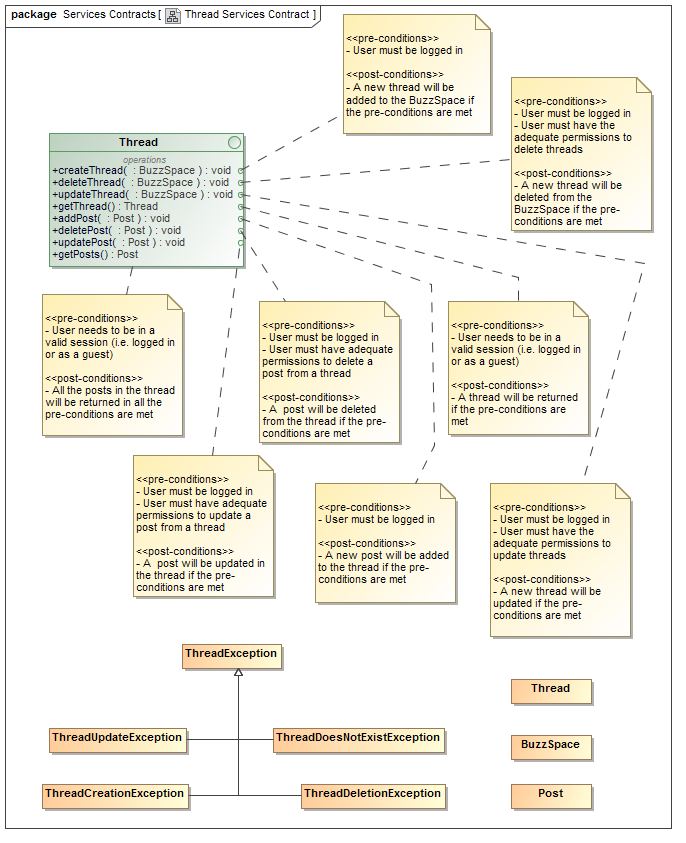
\includegraphics[width=1.0\textwidth]{ThreadSC.png}
				\large\textbf{\colorbox{green}{IMAGE OF ThreadSC}}
				\caption{Tagging services contracts.}
			\end{figure}	
		\subsubsection{Thread Posts}
		\begin{figure}[H]
			\centering
			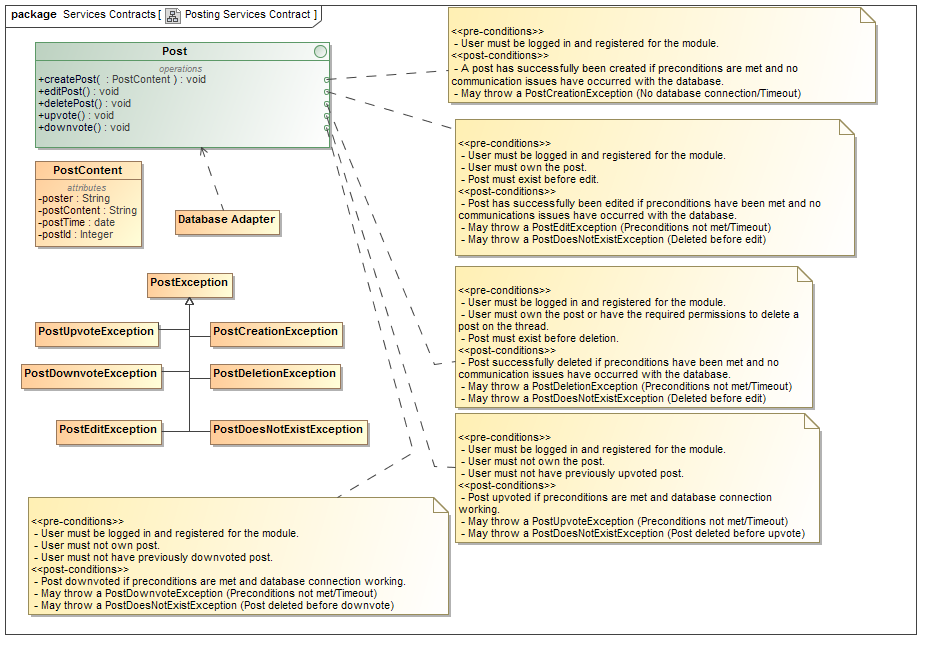
\includegraphics[width=1.0\textwidth]{ThreadPostsSC.png}
			\caption{Thread Posts services contracts.}
		\end{figure}	
		\subsubsection{User}
			\begin{figure}[H]
				\centering
				%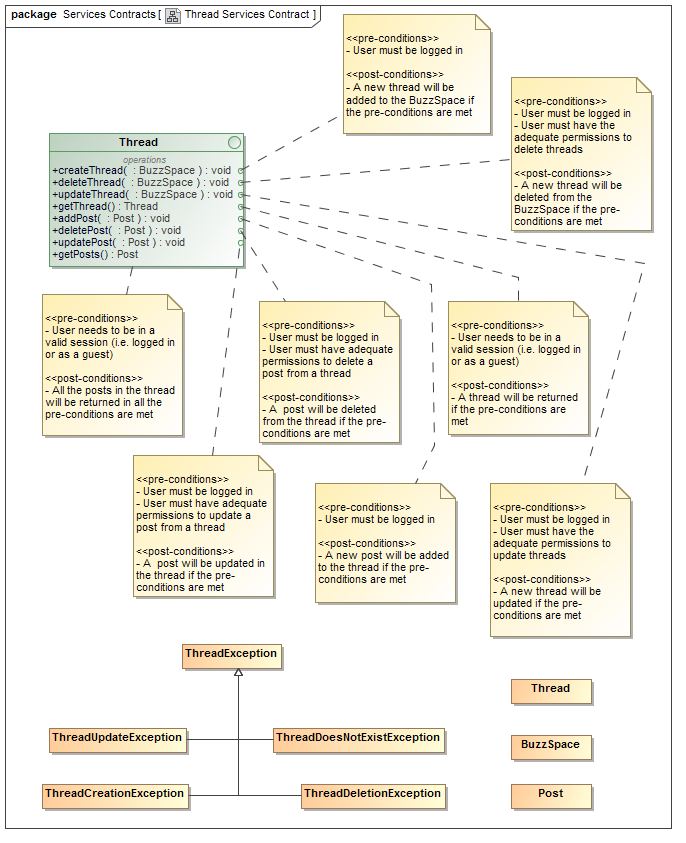
\includegraphics[width=1.0\textwidth]{ThreadSC.png}
				\large\textbf{\colorbox{green}{IMAGE OF UserSC}}
				\caption{Tagging services contracts.}
			\end{figure}
\pagebreak
	\subsection{Required functionality}
		\subsubsection{Analytics}
			\begin{figure}[H]
				\centering
				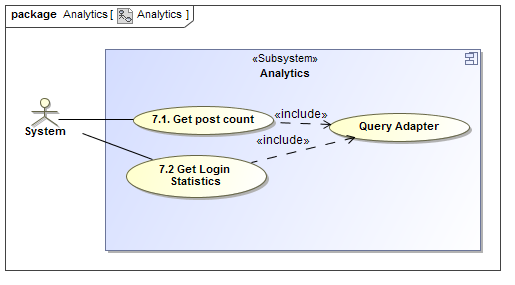
\includegraphics[width=1.0\textwidth]{AnalyticsUC.png}
				\caption{Analytics sub system use case diagram.}
			\end{figure}
		\subsubsection{Authentication}
			\begin{figure}[H]
				\centering
				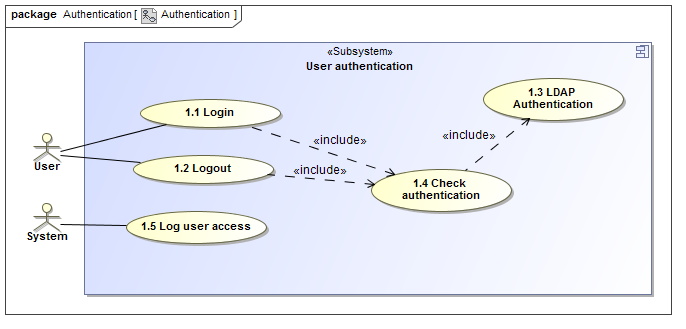
\includegraphics[width=1.0\textwidth]{AuthenticationUC.png}
				\caption{Authentication sub system use case diagram.}
			\end{figure}
		\subsubsection{BuzzSpace}
			\begin{figure}[H]
				\centering
				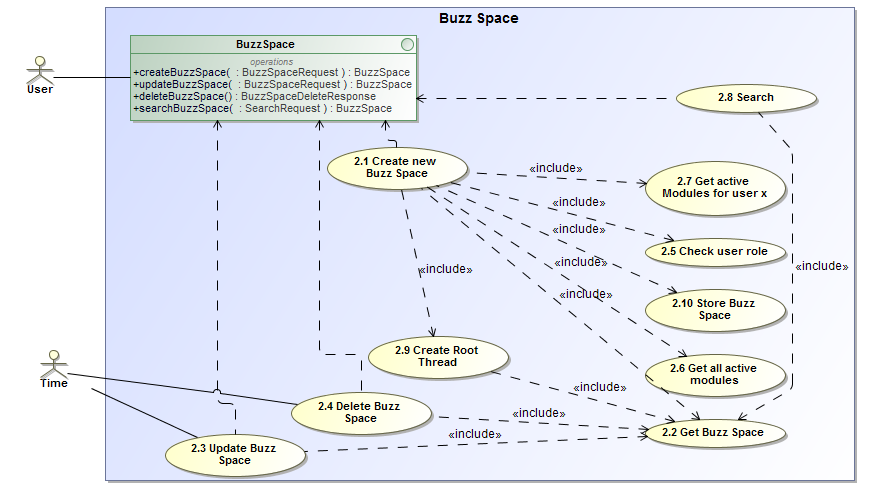
\includegraphics[width=1.0\textwidth]{BuzzSpaceUC.png}
				\caption{BuzzSpace sub system use case diagram.}
			\end{figure}
		\subsubsection{Communication}
			\begin{figure}[H]
				\centering
				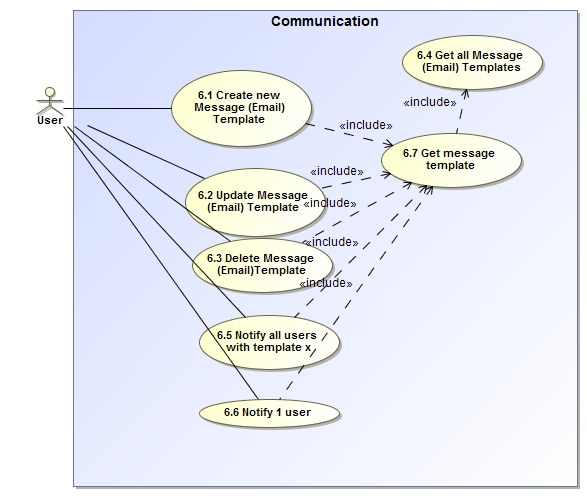
\includegraphics[width=1.0\textwidth]{CommunicationUC.png}
				\caption{Communication sub system use case diagram.}
			\end{figure}
		\subsubsection{Plagiarism / Netetiquette}
			\begin{figure}[H]
				\centering
				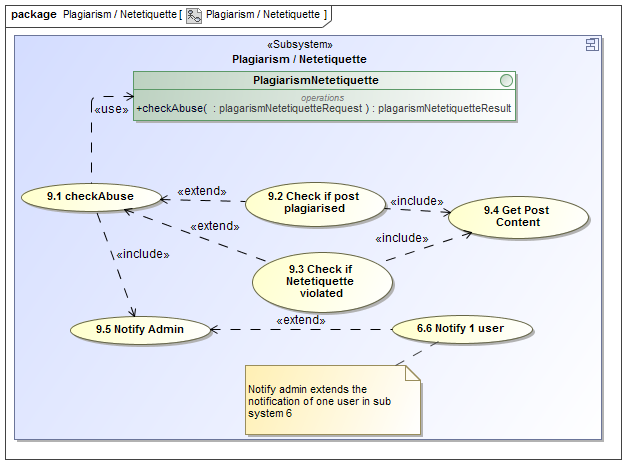
\includegraphics[width=1.0\textwidth]{PlagiarismNetetiquetteUC.png}
				\caption{Plagiarism and Netetiquette sub system use case diagram.}
			\end{figure}
		\subsubsection{Tagging}
			\begin{figure}[H]
				\centering
				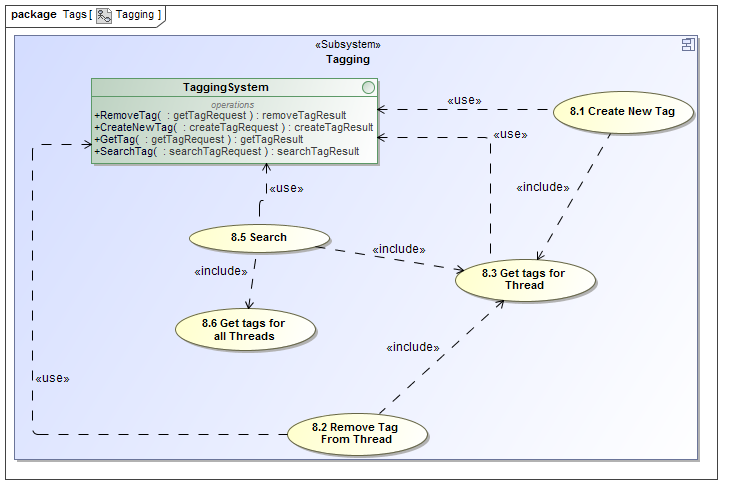
\includegraphics[width=1.0\textwidth]{TaggingUC.png}
				\caption{Tagging sub system use case diagram.}
			\end{figure}
		\subsubsection{Thread}
			\begin{figure}[H]
				\centering
				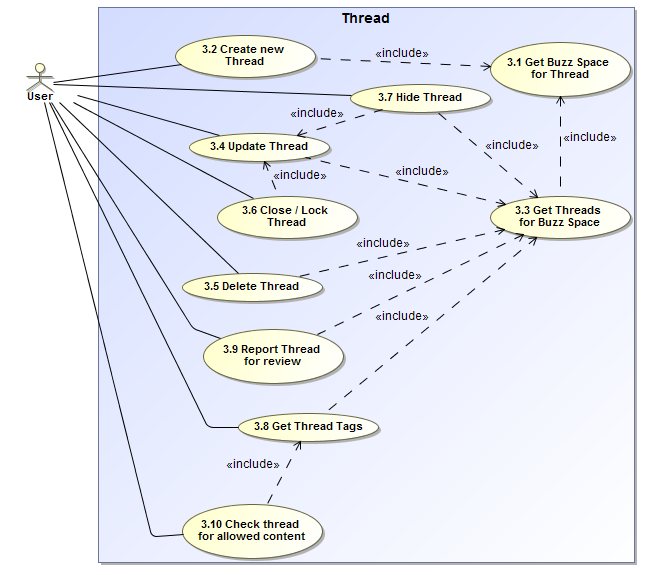
\includegraphics[width=1.0\textwidth]{ThreadUC.png}
				\caption{Tagging sub system use case diagram.}
			\end{figure}	
		\subsubsection{Thread Posts}
			\begin{figure}[H]
				\centering
				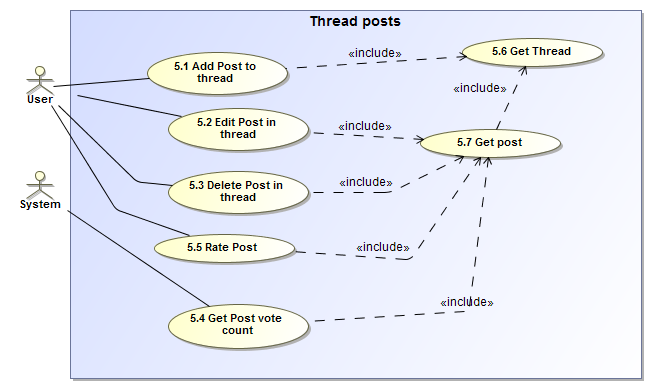
\includegraphics[width=1.0\textwidth]{ThreadPostsUC.png}
				\caption{Thread Posts sub system use case diagram.}
			\end{figure}	
		\subsubsection{User}
			\begin{figure}[H]
				\centering
				\includegraphics[width=1.0\textwidth]{USerUC.png}
				\caption{Tagging sub system use case diagram.}
			\end{figure}
\pagebreak
	\subsection{Process specifications}
		\subsubsection{Authentication}
			\begin{figure}[H]
				\centering
				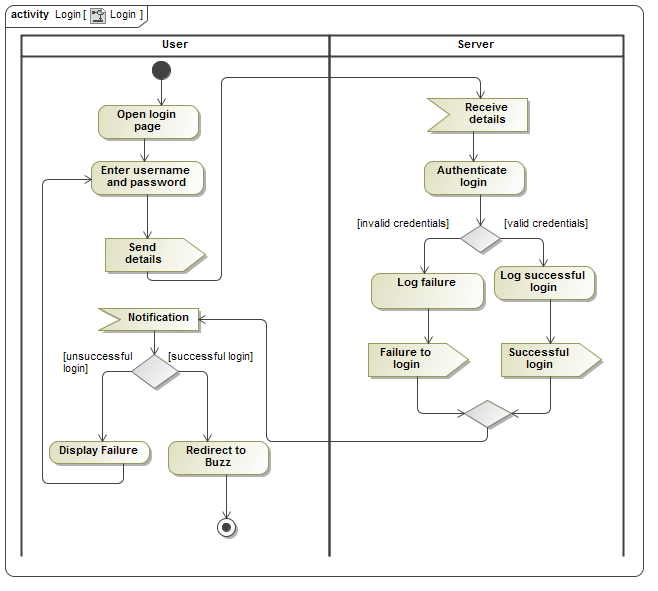
\includegraphics[width=1.0\textwidth]{LoginAD.png}
				\caption{Loign activity diagram.}
			\end{figure}
			\begin{figure}[H]
				\centering
				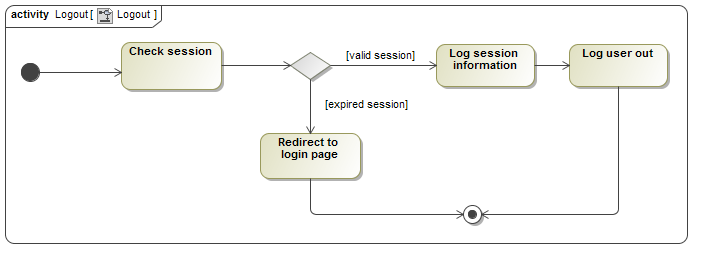
\includegraphics[width=1.0\textwidth]{LogoutAD.png}
				\caption{Logout activity diagram.}
			\end{figure}			
		\subsubsection{BuzzSpace}
			\begin{figure}[H]
				\centering
				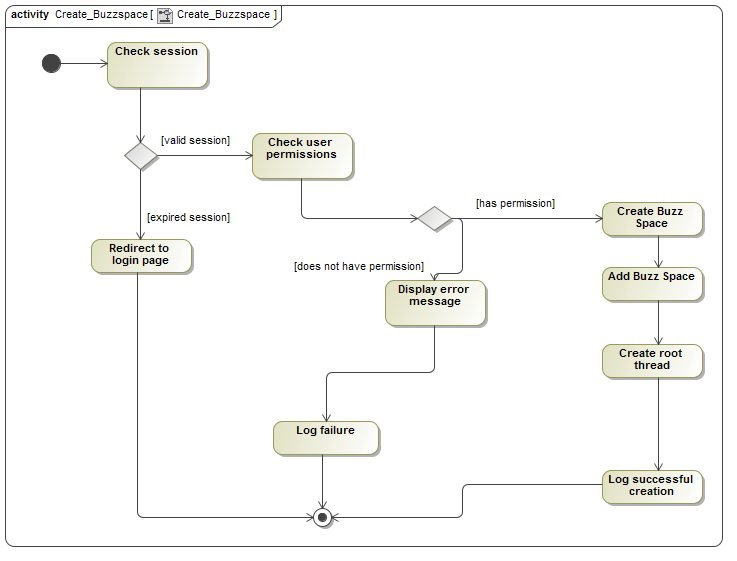
\includegraphics[width=1.0\textwidth]{CreateBuzzspaceAD.png}
				\caption{Create Buzzspace activity diagram.}
			\end{figure}
			\begin{figure}[H]
				\centering
				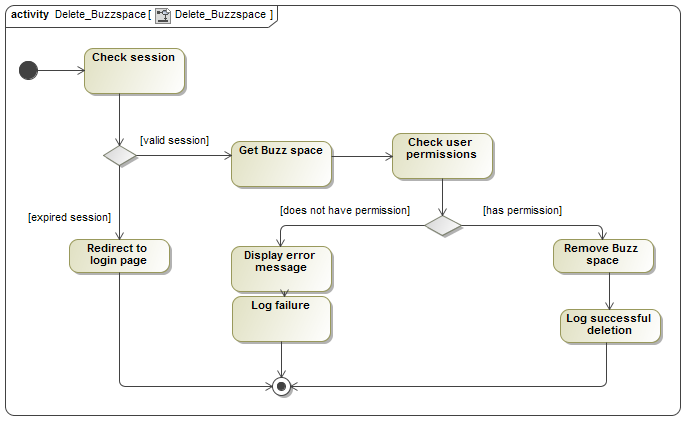
\includegraphics[width=1.0\textwidth]{DeleteBuzzspaceAD.png}
				\caption{Delete Buzzspace activity diagram.}
			\end{figure}
			\begin{figure}[H]
				\centering
				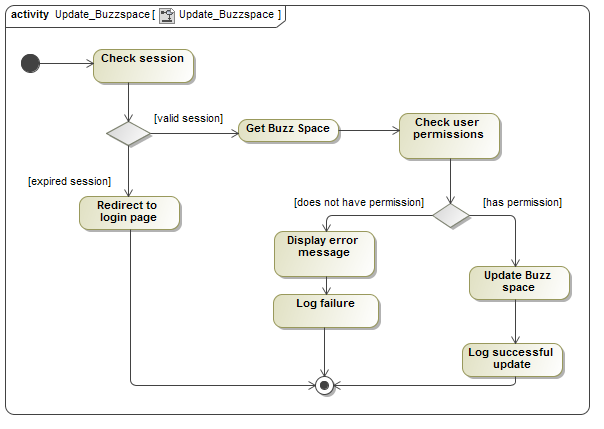
\includegraphics[width=1.0\textwidth]{UpdateBuzzspaceAD.png}
				\caption{Update Buzzspace activity diagram.}
			\end{figure}
		\subsubsection{Communication}
			\begin{figure}[H]
				\centering
				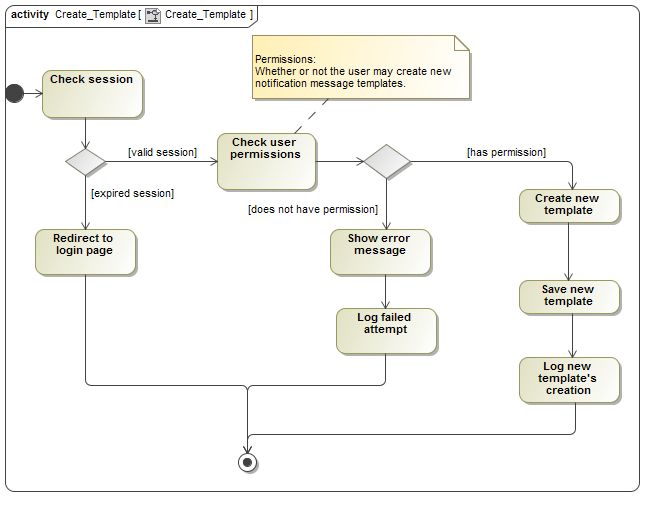
\includegraphics[width=1.0\textwidth]{CreateTemplateAD.png}
				\caption{Create Template activity diagram.}
			\end{figure}
			\begin{figure}[H]
				\centering
				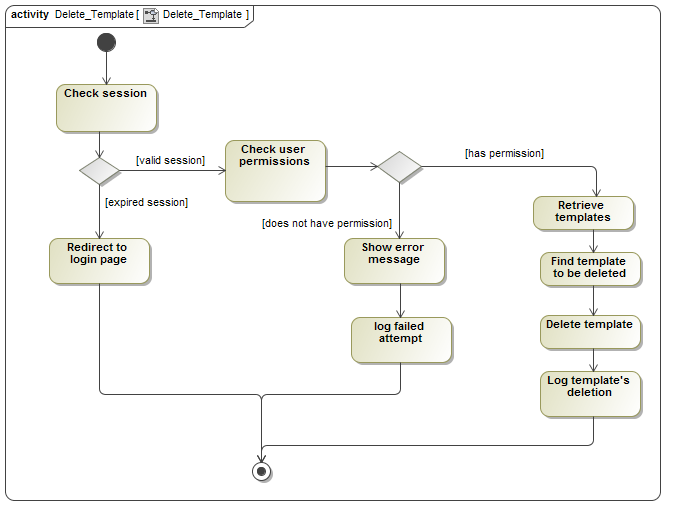
\includegraphics[width=1.0\textwidth]{DeleteTemplateAD.png}
				\caption{Delete Template activity diagram.}
			\end{figure}
			\begin{figure}[H]
				\centering
				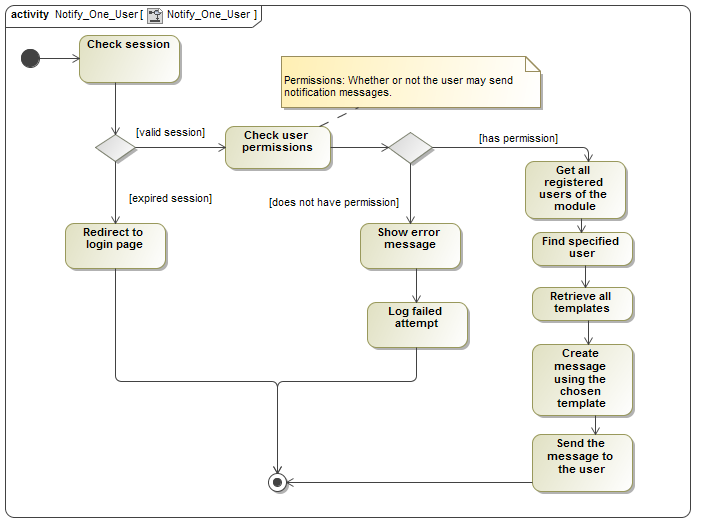
\includegraphics[width=1.0\textwidth]{NotifyOneUserAD.png}
				\caption{Notify One User activity diagram.}
			\end{figure}
			\begin{figure}[H]
				\centering
				\includegraphics[width=1.0\textwidth]{NotifyUSersAD.png}
				\caption{Notify Users activity diagram.}
			\end{figure}
			\begin{figure}[H]
				\centering
				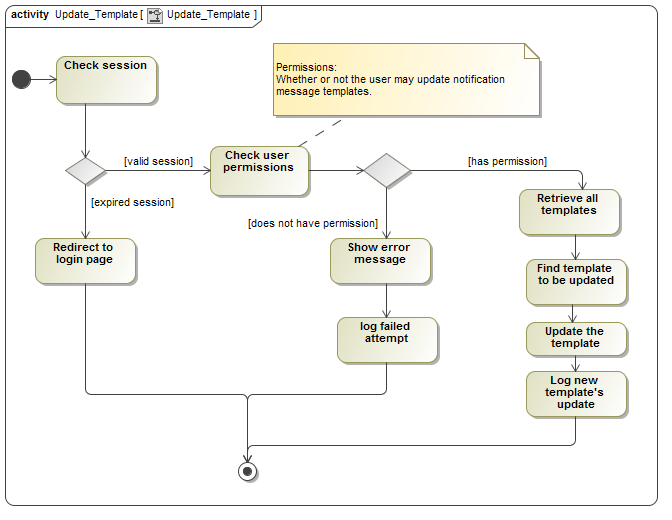
\includegraphics[width=1.0\textwidth]{UpdateTemplateAD.png}
				\caption{Update Template activity diagram.}
			\end{figure}
		\subsubsection{Tagging}
			\begin{figure}[H]
				\centering
				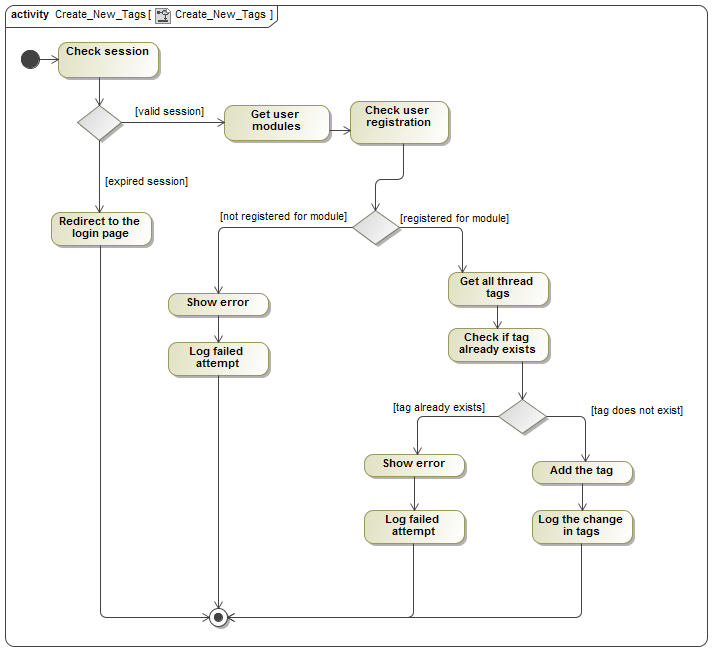
\includegraphics[width=1.0\textwidth]{CreateNewTagsAD.png}
				\caption{Create New Tags activity diagram.}
			\end{figure}
			\begin{figure}[H]
				\centering
				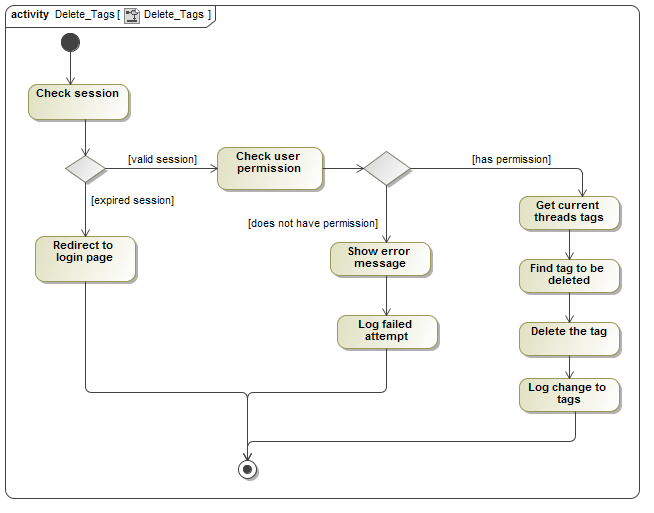
\includegraphics[width=1.0\textwidth]{DeleteTagsAD.png}
				\caption{Delete Tags activity diagram.}
			\end{figure}
			\begin{figure}[H]
				\centering
				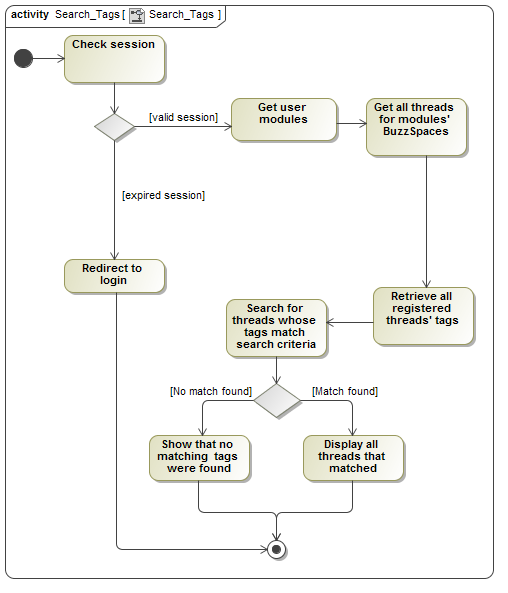
\includegraphics[width=1.0\textwidth]{SearchTagsAD.png}
				\caption{Search Tags activity diagram.}
			\end{figure}
		\subsubsection{Thread}
			\begin{figure}[H]
				\centering
				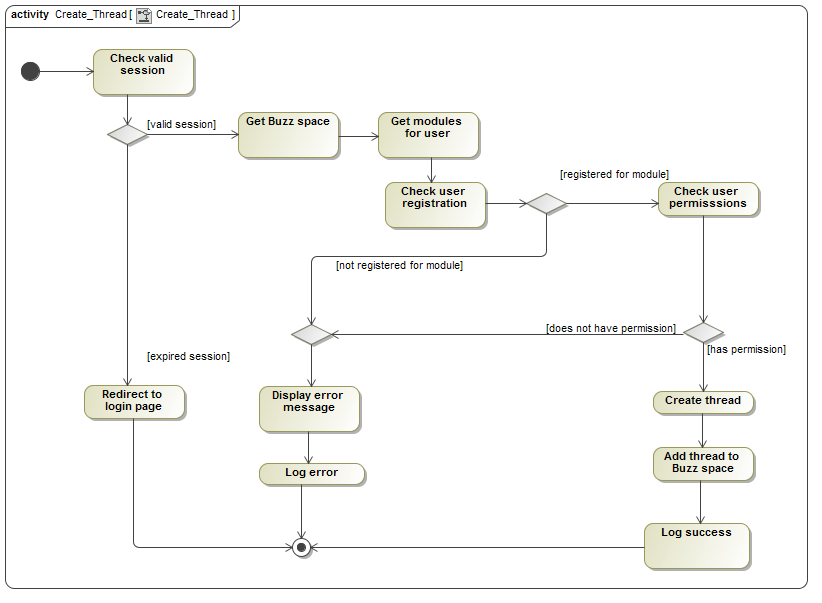
\includegraphics[width=1.0\textwidth]{CreateThreadAD.png}
				\caption{Create thread activity diagram.}
			\end{figure}
			\begin{figure}[H]
				\centering
				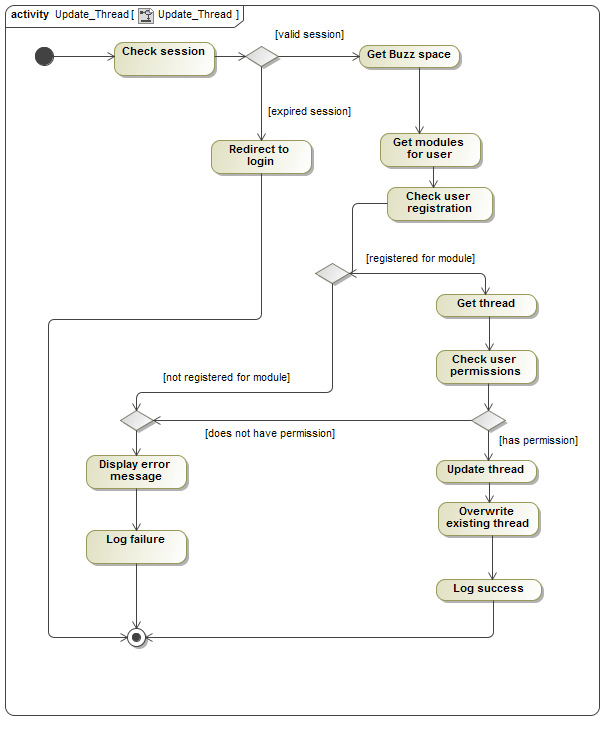
\includegraphics[width=1.0\textwidth]{UpdateThreadAD.png}
				\caption{Update thread activity diagram.}
			\end{figure}               
			\begin{figure}[H]
				\centering
				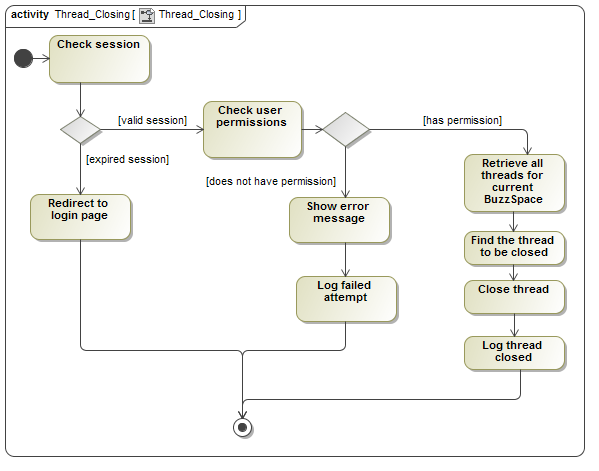
\includegraphics[width=1.0\textwidth]{ThreadClosingAD.png}
				\caption{Close thread diagram.}
			\end{figure}
		\subsubsection{Thread posts}
			\begin{figure}[H]
				\centering
				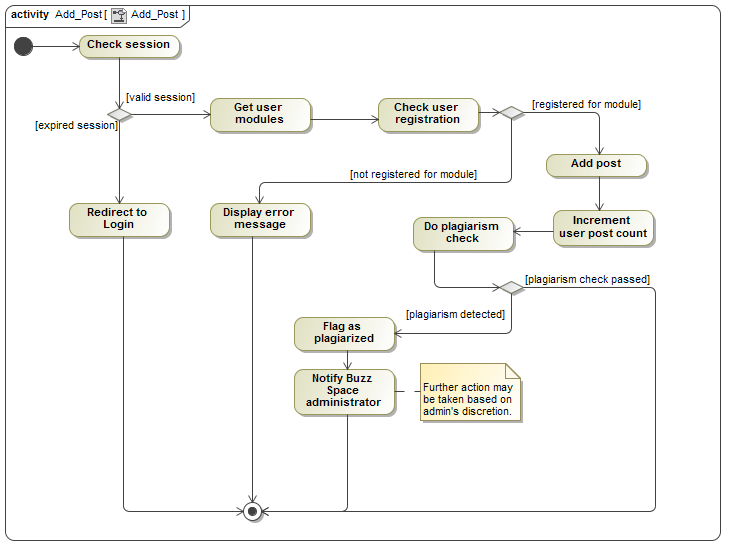
\includegraphics[width=1.0\textwidth]{AddPostAD.png}
				\caption{Add post to thread activity diagram.}
			\end{figure}
			\begin{figure}[H]
				\centering
				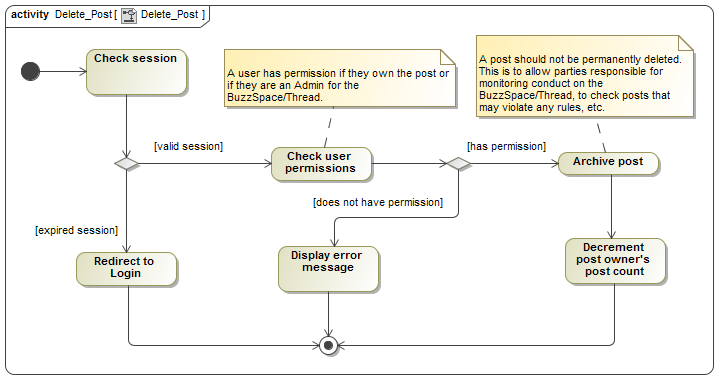
\includegraphics[width=1.0\textwidth]{DeletePostAD.png}
				\caption{Delete thread post activity diagram.}
			\end{figure}
			\begin{figure}[H]
				\centering
				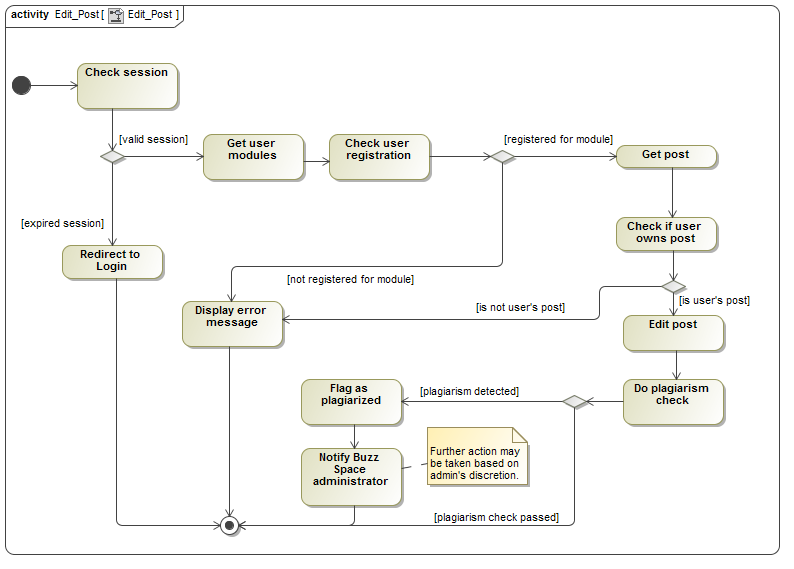
\includegraphics[width=1.0\textwidth]{EditPostAD.png}
				\caption{Edit thread post activity diagram.}
			\end{figure}
			\begin{figure}[H]
				\centering
				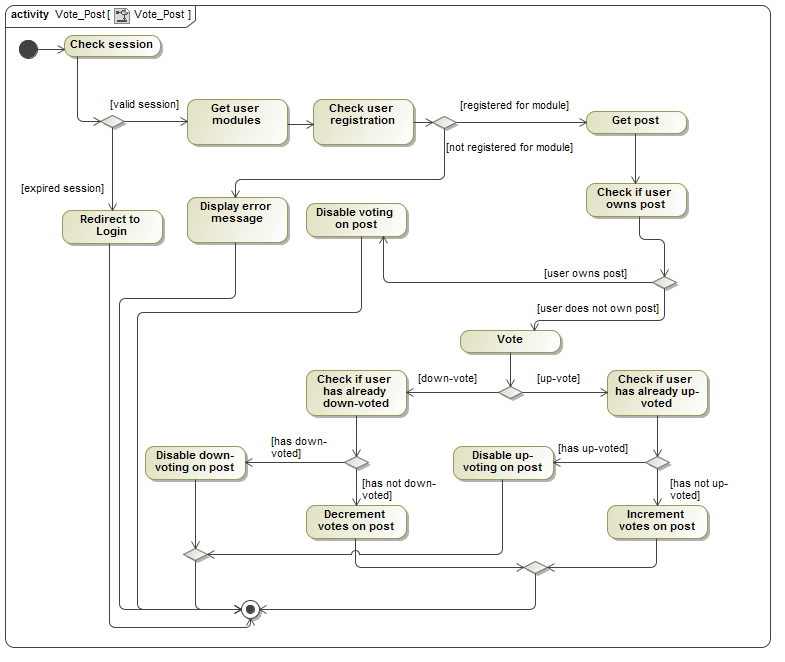
\includegraphics[width=1.0\textwidth]{VotePostAD.png}
				\caption{Vote for post activity diagram.}
			\end{figure}

\pagebreak
	\subsection{Domain Model}
		\begin{figure}[H]
			\centering
			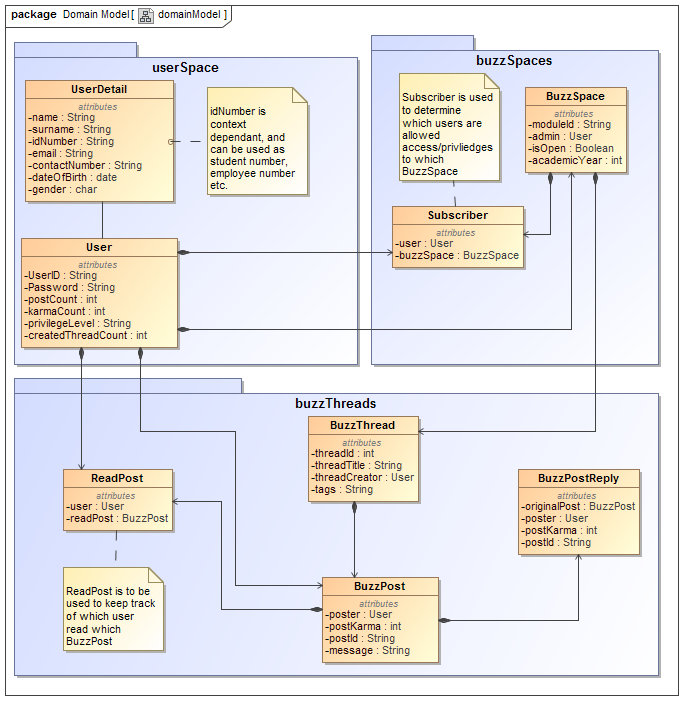
\includegraphics[width=1.0\textwidth]{domainModel.png}
			\caption{Domain model for the discussion board.}
		\end{figure}

\end{document}
